% outline introduction
% 1. Reinforcement learning introduction
% 2. games as virtual learning environment
% 3. Research approach
% 4. Structure of the Dissertation

\chapter{Introduction}

Artificial Intelligence is an extremely interesting but difficult problem to
address, as research has to at least account for the complexity and breath of
behaviour that has been shown in animals and humans. Autonomy can be sometimes
programmatically engineered, but most of intelligent behaviour requires some
amount of learning that can only be acquired through direct interaction with the
environment. A big part of being ``intelligent'' has to do with the ability
to generalise knowledge and behave reasonably in unseen scenarios, which makes
formalising and tackling the general problem nearly impossible.

\section{Reinforcement Learning}

A technique developed specifically to address this type of learning process is
Reinforcement learning. Reinforcement learning provides a general framework in
which to learn behaviour in a goal-oriented fashion and without requiring expert
knowledge or labelled data. It is framed to be functional even in situations
where reward is delayed and where environments are not deterministic. Because of
its foundations on dynamic programming, it also allows the use of rich and
powerful mathematical tools for its analysis. Unfortunately those algorithms
learn more or less good behaviour only when the environment is sufficiently
tractable, and they start breaking down as the state space increases in size. To
study reinforcement learning we therefore need testbeds that allow to
parametrise the size of this state and that remain interesting enough to provide
challenges for evolving state-of-the-art algorithms.

\section{Games as Virtual Learning Environments}

The idea of using games as testbeds for Artificial Intelligence is certainly not
a new one. Chess, Backgammon, Go and various other board games have historically
been linked to challenges and advances in AI research, and the AI community has
used those games to compare and study the properties of different algorithms.

During the past couple of decades the community has gradually ``solved'' or
fully tackled most of those board games, leaving researchers with fewer
available platforms and generally too large domains for structural analysis not
to construct additional research problems. On the other hand, the surge of
computer games provided the community a perfect excuse to study search
algorithms and symbolic solvers because of the need to challenge human players,
allowing at least part of the community to steadily keep working.

\begin{figure}[h]
    \centering
    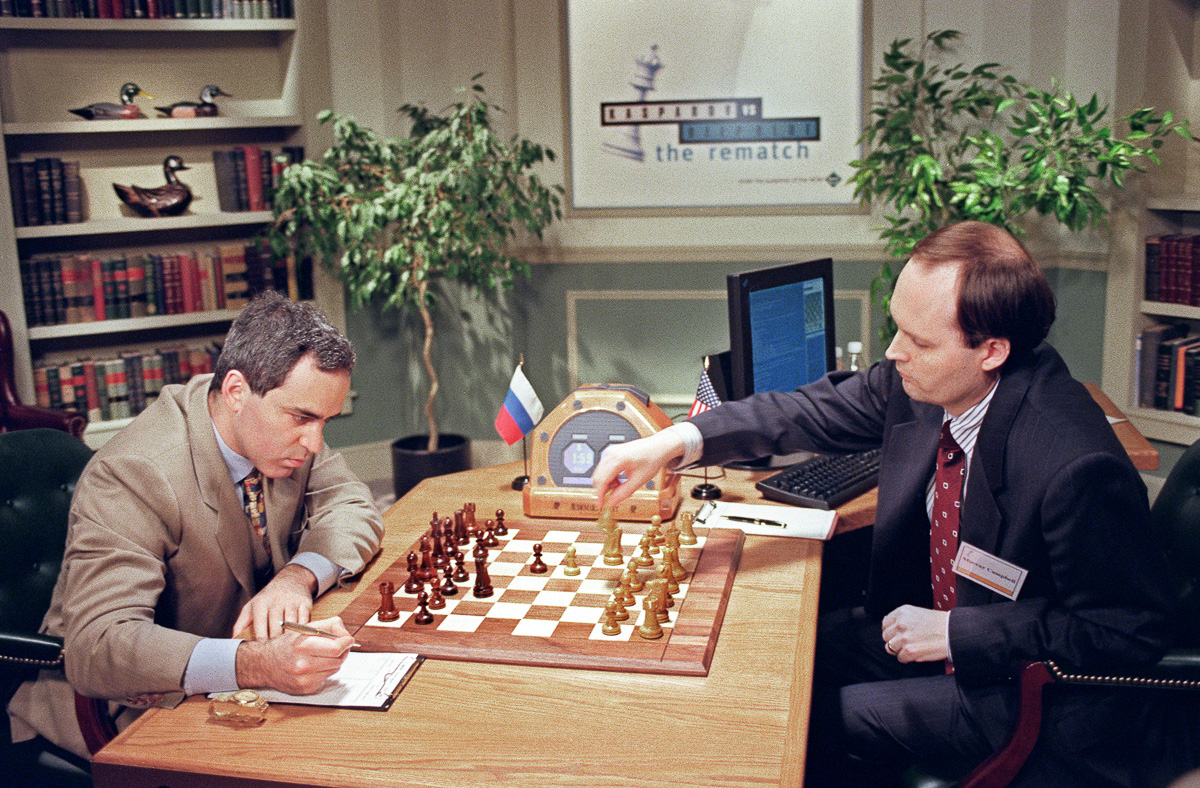
\includegraphics[width=0.9\textwidth]{ch1/kasparovdeepblue}
    \caption{May 1997. IBM scientist Murray Campbell, makes a move for Deep Blue
      in the second game of the historical match. (Image: Stan Honda / AFP /
      Getty Images)}
    \label{fig:kasparovdeepblue}
\end{figure}

Reinforcement Learning algorithms have since the beginning found usage when
applied to fields such as robot control, natural language processing and
economics, but most of the theoretical work has required the usage of relatively
simple and scalable testbeds to develop and compare algorithms in a systematic
and rigorous manner. Most of those domains consisted in direct adaptations of
classical AI problems such as grid worlds and bandit problems, but as research
started getting past those simple domains the community had to come up with more
structured and complex environments. However providing a strong justification
for building solutions for platforms customised and designed to provide
particular levels of difficulty was never terribly easy.

Those testbeds have as well historically mostly consisted of board games like go
and backgammon, but in the past couple of decades the community has started
popularising domains such as simulated football, autonomous racing and a variety
of computer games as suitable platforms for research in decision making. All of
those share characteristics that make naive reinforcement learning complex to
engineer and train: they can possess large action or environment state spaces,
they challenge algorithms by providing only a degree of partial observability or
they can be properly tackled only by obtaining strong long-term strategies (with
complexity more suitable for communities like symbolic planning and search).

\begin{figure}[h]
    \centering
    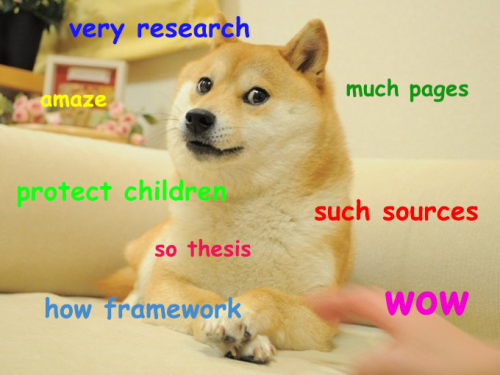
\includegraphics[width=\textwidth]{placeholder}
    \caption{The ATARI Learning Environment.}
    \label{fig:ALE}
\end{figure}

An example of a recent popular learning platform is the Atari Learning
Environment (ALE), which researchers have mostly used to study reinforcement
learning algorithms that can learn a variety of policies for different games of
various complexity. Unfortunately the majority of the games contained in this
particular platform don't necessarily require anything way more complex than
reactive policies, which means that studying more advanced policy learning on
those games has become quite a forced process.

A category of computer games instead more suitable for providing complex
scenarios for studying RL is the category of Real-Time Strategy (RTS) games.
This typology of games generally requires some amount of long-term planning
combined with interactive and generalisable short-term (and reactive) planning,
with the complexity becoming almost entirely context-dependent, as it is often
the case in real-life scenarios. Those are particularly challenging to existing
classical reinforcement learning algorithms because of the often intrinsic
partial observability, the unusually big action space, and their nature of
competitive game which makes modelling adversarial processes almost a
requirement. In this thesis we focus on one of the most popular and still widely
played RTS games, StarCraft.

% cite from http://umichrl.pbworks.com/w/page/7597597/Successes%20of%20Reinforcement%20Learning

\section{Thesis Work} % TODO rename

The point of this work was primarily about exploring what it would take to
concretely transform and use StarCraft as a platform to study reinforcement
learning and general artificial intelligence. We adopted a scoping approach to
deal with the engineering problem, with the goal to reach a state where we could
successfully run state of the art learning algorithms on StarCraft. This brought
us to design and develop a robust and generic interface to the game using some
existing tools, the creation of an interface to one of the popular tensor
libraries and finally porting and testing a few basic reinforcement learning and
deep reinforcement learning algorithms.

The idea was to prove the feasibility of using StarCraft as a learning platform,
to release the first version of a useful interface to allow the community to
bootstrap work on real-time strategy games, and to create a baseline for later
work in the area.

\section{Report Structure}

Chapter 2 presents reinforcement learning and discusses some of the research
done on computer games. We outline properties of real-time strategy games and we
seek to explain the benefits of using StarCraft as a research platform. Chapter
3 presents the engineering approach taken and the developed architecture,
covering the entire pipeline from the game to the agent interface, also
providing some example agent learning algorithms. Chapter 4 presents results
obtained from testing the platform using a couple of model-free reinforcement
learning algorithms. Finally Chapter 5 discusses some improvements for the
design and future work.
